\documentclass[conference]{IEEEtran}
\IEEEoverridecommandlockouts


% 包引用
\usepackage{cite}
\usepackage{amsmath,amssymb,amsfonts}
\usepackage{algorithmic}
\usepackage{graphicx}
\usepackage{epstopdf}
\usepackage{textcomp}
\usepackage{xcolor}
\def\BibTeX{{\rm B\kern-.05em{\sc i\kern-.025em b}\kern-.08em
    T\kern-.1667em\lower.7ex\hbox{E}\kern-.125emX}}

% 图片路径
\graphicspath{{figure/}}

% 正文
\begin{document}

% 标题
\title{Privacy-Preserving Multi-hop Payments with Constant Collateral}

% 作者
\author{\IEEEauthorblockN{1\textsuperscript{st} Given Name Surname}
\IEEEauthorblockA{\textit{dept. name of organization (of Aff.)} \\
\textit{name of organization (of Aff.)}\\
City, Country \\
email address or ORCID}
\and
\IEEEauthorblockN{2\textsuperscript{nd} Given Name Surname}
\IEEEauthorblockA{\textit{dept. name of organization (of Aff.)} \\
\textit{name of organization (of Aff.)}\\
City, Country \\
email address or ORCID}}

\maketitle

\begin{abstract}
This document is a model and instructions for \LaTeX.
\end{abstract}

\begin{IEEEkeywords}
component, formatting, style, styling, insert
\end{IEEEkeywords}

\section{Introduction}
In recent years, permissionless cryptocurrencies, have emerged as a novel means to facilitate secure
and reliable payments within a decentralized framework, garnering significant attention from both academia 
and industry. These cryptocurrencies employ a consensus mechanism to verify each transaction, which is
then recorded on a publicly distributed ledger known as blockchain. Unfortunately, 
the widespread adoption of cryptocurrencies is hindered by notable scalability challenges. 
Complex consensus mechanisms, like Bitcoin's Proof-of-work(PoW), and the limited block size of the 
blockchain contribute to the issue. The theoretical throughput of Bitcoin stands at approximately 10 transactions 
per second(TPS), with a transaction confirmation time of around 1 hour. In contrast, traditional decentralized 
payment networks, such as Visa, boast the capability up to 47,000 TPS. Furthermore, the presence of high 
transaction fees renders small-value payments impractical for cryptocurrency users. 

One promising solution proposed to address the scalability issue is the utilization of payments channels(PCs), 
which facilitate quick and validated transactions between two parties off-chain. In a nutshell, a payment 
channel is represented as a multi-signature address on the blockchain, with both parties initially depositing 
a certain amount of funds. Subsequently, during each transaction, the parties adjust the fund allocation by 
generating and exchanging signed transaction messages off-chain. When the participants decide to settle the 
channel or encounter a dispute, they initiate the closing process by broadcasting the latest signed transaction to the blockchain. 

However, this straightforward construction forces users to establish a separate payment channel with each
potential transaction partner and lock coins for each one. Additionally, these coins cannot be used for other 
things until the channel is closed. Payment channel network(PCN) mitigates this issue by enabling transactions 
between two users who do not share a direct payment channel. This is achieved through multi-hop payments(MHP) 
by leveraging intermediaries and payment channels within the PCN.

\subsection{PCN based on HTLC and some limitations}
Currently, the most renowned and valuable PCN system is the Lightning Network(LN), which is implemented on 
the Bitcoin. To guarantee the security and atomicity of multi-hop payments, LN employs a specialized mechanism 
called hash timed-locked contracts(HTLCs). The HTLC mechanism involves two phases. In the locking phase, coins 
are locked in each channel using a hash chosen by the receiver from the left to right. In the subsequent release 
phase, the receiver present the preimage of the hash value he initially selected to unlock coins and all the 
intermediaries can claim coins by providing the same preimage. An example of a MHP based HTLC is shown in figure 1. 
Unfortunately, PCNs based on HTLC have the following fundamental problems.

\begin{figure}[b]
	\centering
	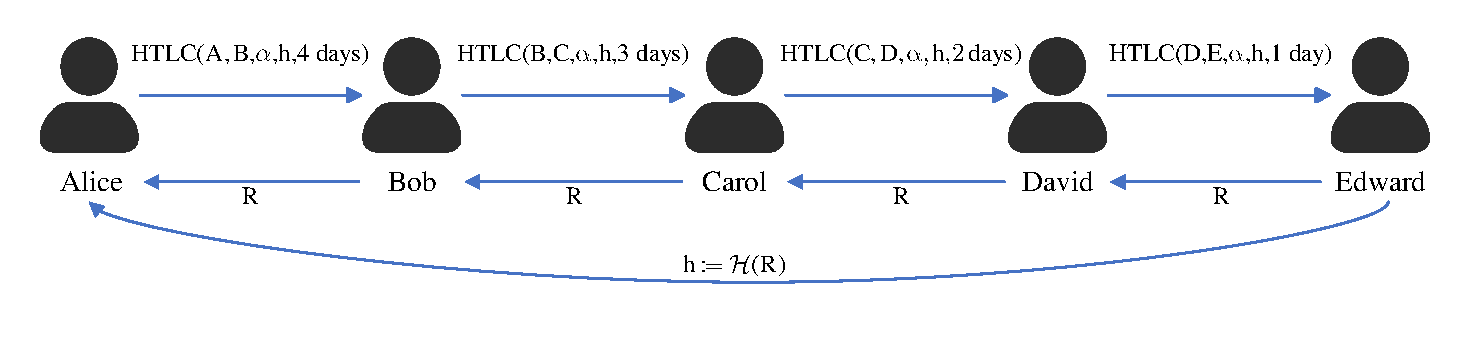
\includegraphics[scale=0.35]{htlc.pdf}
	\caption{An MHP from Alice to Bob for value $\alpha$ coins using HTLC contracts. A HTLC contract denotes as 
		HTLC(X, Y, $h, \alpha, t$) means:(i)If Y can present a value $r$ such that $\mathcal{H}(r)=h$ before timeout $t$,
		X pays $\alpha$ coins to Y.(ii)If timeout $t$ expires, X gets back the $\alpha$ locked coins}
\end{figure}

\textbf{Collateral} To ensure the atomic execution of MHP, each HTLC needs to specify an expiration time(also called 
collateral time) for the locked coins. Once time expires, the locked coins will be returned to the user on the left 
side of the channel. Moreover, the collateral time increases gradually from left to right in a staggered fashion. 
Assuming $\alpha$ coins are being paid through $\emph{n}$ PCs, the collateral time for PC $\emph{i}$ is $\emph{t}_{\emph{i}}\geq\emph{t}_{\emph{i}}+\Delta$, 
$\emph{i}=1,2,\cdots ,\emph{n}$, $\Delta$ denotes the maximum duration between when a transaction is broadcast and 
when it is confirmed transaction by the blockchain. This staggered manner ensures that each user has enough time to 
await the timely update of his right channel and expeditiously broadcast the state of his left channel to the blockchain, 
regardless of whether the counterparty cooperates. 

While this mechanism effectively prevent honest users losing coins, it is essential to note that the overall collateral 
for the entire payment path is $\Theta \left ( \emph{n}^{2}\cdot \alpha\cdot  \Delta  \right )$ in the worst-case 
scenario in units $ \emph{coins}\times \emph{time}$. In the event of a failure of the MHP where all coins are returned, 
users cannot receive any benefit but incur potential financial losses. This is due to the fact that the locked coins 
cannot be utilized for other transactions during this period. Furthermore, the high volatility of cryptocurrency 
prices can exacerbate these economic losses, further magnifying the impact on users' financial well-being. 
Simultaneously, it is crucial to acknowledge that this issue is not limited to the HTLC mechanism alone, 
but rather applies to all multi-hop payments protocols within two-phase communication \cite{blitz}. 

\textbf{Anonymity} Despite the employment of onion routing \cite{onion routing}, \cite{sphinx} for anonymity in 
the LN, it is important to be aware that the information contained in HTLCs can inadvertently expose details 
about payment path. In our analysis, we examine the inherent limitations of the HTLC mechanism regarding anonymity 
from both \textit{off-chain} and \textit{on-chain} perspectives. 

\section{Background}
In this section, we provide an overview on the background and the notations used throughout the paper.

\subsection{UTXO model}
In this work, we assume the underlying blockchain, like Bitcoin, is based on the UTXO model. Transaction output is 
the fundamental component of Bitcoin transaction, which is an indivisible Bitcoin currency recorded on the blockchain 
and recognized as valid by the entire network. The Bitcoin complete nodes tracks all available outputs called 
\emph{unspent transaction outpus} (UTXO). UTXOs can be any value and once generated are indivisible, a UTXO can only 
be consumed as a whole in a single transaction. The output consists of two parts, which we represent as a 
tuple $\theta :=\{cash,\phi\}, \theta.cash$ is the output value, and the $\theta.\phi$ is the condition to spend 
this output, it also called \emph{locking script}. Onesig(\emph{U}) indicates that the condition required to 
spend this output is a digital signature. We say that a user \emph{U} can spend an output only if $\theta.\phi$ 
contains only a signature w.r.t verification  \emph{U}'s public key, if multiple signatures are required, we use 
MultiSig($\it U_1,U_2,...,U_n$).

% UTXO model
\begin{figure}[t]
	\centering
	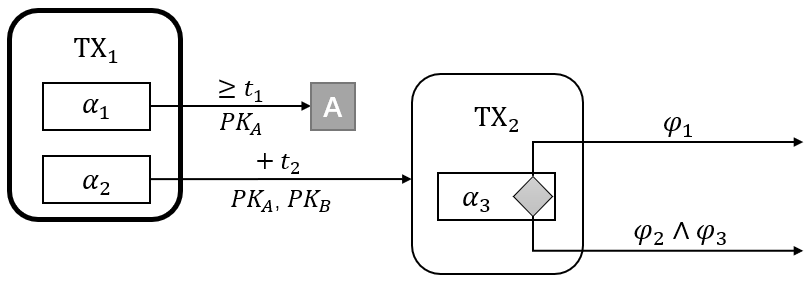
\includegraphics[scale=0.5]{fig2.png}
	\caption{Left transaction $TX_1$ is recorded on the blockchain, which has two output. Value $\alpha_1$ can be spent 
	by A, with a transaction signed w.r.t $PK_A$ after $\emph{t}_1$ rounds, and the output of value $\alpha_2$ can 
	be spent by a transaction signed w.r.t $PK_A$ and $PK_B$ but only if at least $\emph{t}_2$ rounds has passed 
	through after the transaction being published on the blockchain. The right transaction $TX_2$ has one input 
	which is the second output of $TX_1$ with the value $\alpha_1$. $TX_2$ has only one output containing $\alpha_3$ 
	coins, which can spent by a transaction whose witness satisfies the condition $\varphi_1 \vee (\varphi_2 \wedge \varphi_3)$}
\end{figure}

Transactions consume previously recorded unused UTXOs and create new UTXOs available for future transaction, in this 
way, the transaction continues in the form of a chain of owners. on the chain, the input of the transaction corresponds 
to the output of the previous transaction. We denote a transaction as a tuple TX := \{id,input,output,timelock,witness\}, 
TX.id$\in\{0,1\}^*$ is the identifier of a transaction and TX.id = $\mathcal H$(TX.input,TX.output,TX.timelock), $\mathcal H$ 
is a hash function, modeled as a random oracle. TX.input and TX.output denotes the list of the inputs and the list of 
new outputs respectively. $\bf TX$.timelock defined as the earliest time a transaction is valid and can be transmitted 
on the network or added to the blockchain, it defaults to 0 in most transactions. TX.witness$\in\{0,1\}^*$, also 
called \emph{ScriptSig}, is part of the transaction input to address or satisfy the spending conditions set by the 
\emph{locking script} on the output. Actually, before being recorded on the blockchain, transactions must go through 
the consensus mechanism of all nodes. During this period, each node will independently verify the transaction. 
Transactions need to be verified as follows: For a transaction(1) The sum of the input value cannot be less 
than the sum of the output value;(2)For each input, the quoted output cannot exist in any other transaction, 
it must exist and not be spent;(3) The \emph{ScriptSig} for each input must be validated against the \emph{locking script} 
for the corresponding output.To put it simply, the transaction must provide valid validation that satisfies the spending 
conditions of each input.

We use charts to visualize the transaction for a clearer illustration. Rounded rectangles represent transactions, 
thick-edged rectangles represent transactions that have already been published on the blockchain, and thin-edged 
rectangles for transactions to be published. The transaction contains at least one box to represent the output 
of the transaction, and the value in the box indicates the number of coins in this output. On the arrows coming 
from the output, are noted the conditions under which this output is spent. The public key below the arrow indicates 
who can use this output; Above the arrow is the timelock for the output(in this work only uses timelock as additional 
condition, which in practice could be any script supported by the underlying blockchain scripting language). There 
are two types of timelocks: \emph{relative time lock} and \emph{absolute time lock}, we use "+\emph{t}" to represent 
the relative time lock, that is, the transaction only vaild at least \emph{t} blocks has passed through after the 
transaction being recorded on the blockchain; The absolute time lock "$\geq$\emph{t}" specifies the absolute time point, 
indicating that the first transaction has passed through \emph{t} round after being recorded on the blockchain. Finally, 
we use a diamond to represent the relationship of "or" that the output conditions are different, expressed in the symbolic 
form as $\varphi = \varphi_1 \vee ...\vee \varphi_n$, where $\varphi$ is the output locking script, written on the arrows 
of the output. A complete example is given in Fig. \colorbox{yellow}{1}.

\subsection{Payments channels}
The payment channel is opened by two users locking some coins on the blockchain, and then the two parties can make as many 
quick instant confirmation transactions off-chain, that is, without waiting for transmitting the transaction to the blockchain, 
as long as the total amount of each transaction is less than the locked value. During the lifetime of the channel, only two 
transactions will be recorded on the blockchain, one is funding transaction $TX_f$ which used to open the channel, the other is 
settlement transaction for close the channel. The funding transaction $TX_f$ determines the balance of this channel, and the 
channel is open when $TX_f$ is broadcast to the network and recorded on the blockchain, both parties update the channel balance 
by exchanging signed transactions off-chain, these transactions holding the reassigned balances are called state of the channel. 
Finally, the channel is closed by posting settlement transaction, which is the final state, on the blockchain. In a more detail, 
there are three operations of the payment channel: $\emph{open, update,}$ and  $\emph{close}$.

1) \emph{Open}: Suppose that Alice and Bob want to create a payment channel, and to do so, Alice and Bob agree on a funding transaction 
$TX_f$. The output value of $TX_f$ is $\alpha_A+\alpha_B$, which is the total amount of the channel, and there are two inputs 
to the $TX_f$ are from Alice and Bob respectively, $\alpha_A$ represents the initial deposit provided by Alice in the channel, 
and $\alpha_B$ represents Bob's. When $TX_f$ is published on the blockchain, it indicates that the payment channel has been opened.

2) \emph{update}: After the channel is opened, to update the balance status of both sides of the channel, that is to make a 
transaction, parties exchange signatures on the commit transaction. Each time a new "commit transaction" is exchanged, the 
previous state of the channel is overwritten and updated to the newer state, while the old state is saved locally. Therefore, 
only the most recent commit transaction can be "executed". To ensure the security of payments, payment channel use a penalty 
mechanism to: 1) prevent malicious user from closing the channel by sending an outdated but self-advantageous state to the chain, 
and 2) enable honest user to acquire all the coins locked in the channel when dishonest user post outdated promised transactions. 
We use the recent work \emph{generalized channels} \colorbox{yellow}{[2]} as the basic structure, which split the "commit transaction" 
into two parts, the commit transaction $TX_c$ responsible for penalizing and the split transaction $TX_s$ that hold the actual output 
of the channel. assume that Alice wants to pay $x_A \leq \alpha_A$ coins to Bob. To do this, they create new commit transaction $TX_c'$ 
and split transaction $TX_s'$, at the same time, they pick the new \emph{secret R'} to represent the commitment of the two parties 
to the new balance of the channel, then they exchange the \emph{revocation secret r} of the previous round of transactions $TX_c$ 
and $TX_s$, after that they make the new commit transaction $TX_c'$ and split transaction $TX_s'$ overwrite previous ones. $TX_s'$ 
represents the updated balance of the channel, and both parties save the previous round of transactions ($TX_c$ and $TX_s$) with the 
\emph{revocation secret r} of the secret value in local memory.

% generalized channels
\begin{figure}[t]
	\centering
	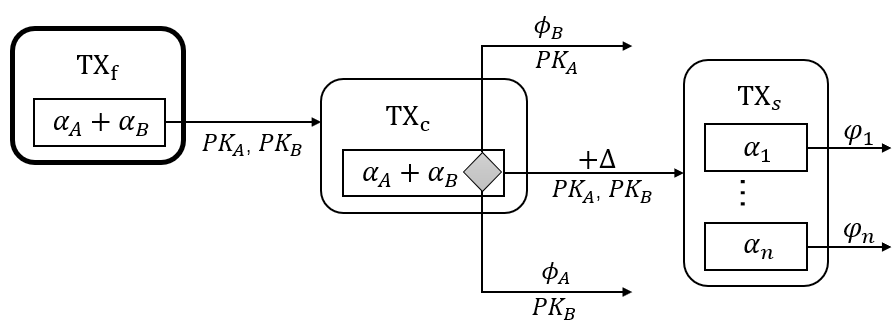
\includegraphics[scale=0.45]{fig3.png}
	\caption{Details of generalized channel, $(x_1,\varphi_1)...(x_1,\varphi_1)$ are the states of the channel. 
	The output of $TX_c$ is three different conditions, two of which are punishment mechanisms used to prevent 
	dishonest users. The condition $\phi_B$ is punishment for B, represents the verification of B’ revocation 
	secret, When A discovers that B submit an old transaction, it can take all the money in the channel by B' 
	revocation secret, which B has exchanged for A when the old transaction is updated. In the same way, $\phi_A$ 
	represents the verification of A’ revocation secret that can punish A. The value of $\Delta$ is time upper 
	bound that takes to publish a transaction on a blockchain.
	}
\end{figure}

3) \emph{close}: Finally, assume both parties agree to close the channel, They can collaboratively submit $\overline{TX_c}$ 
and $\overline{TX_s}$, which represent the last transaction they agreed, to the blockchain to close the channel. If the 
dishonest one submit an expired promised transaction, the malicious party can be penalized by closing the channel through 
the revocation mechanism unilaterally.

\subsection{Payment channel networks}
Suppose that $U_0$ now wants to transfer some coins to $U_2$, but there is no direct payment channel between $U_0$ and $U_2$, 
and instead, there is an indirect path in which $U_1$ participates, that is, $U_0$ has a open payment channel with $U_1$, $U_1$ 
has an open payment channel with $U_2$, then $U_0$ can safely transfer coins to $U_2$ through this path.This way of allowing 
the atomic transfer of coins from the sender to the receiver through intermediaries atomically called \emph{multi-hop payment} (MHP). 
A Payment Channel Network (PCN)\colorbox{yellow}{[1]} is a graph consisted of users as the vertices and edges as channels between 
pairs of users. It can make a large number of single channels connected in series, thus forming an interconnected, vast payment network. 
Any user on the PCN can pay in MHP through a path of open payment channels. 

\noindent $\bf{HTLC}$ However, in the payment process, there is no way to ensure that each user can perform honestly, and malicious 
users will cause honest users to lose coins. To guarantee the atomicity of payments, the Lightning Network (LN)\colorbox{yellow}{[3]} 
is done by using a Hash Time-Lock Contracts (HTLC), which works as follows. In the payment channel of $u_0$ and $u_1$, $u_0$ locks her 
coins in the output, and this output can be spent on two conditions: 1) beyond the predefined time, $u_0$ will get her money back; 
2) once $u_1$ provides a pre-image $r_A$ with a hash value $\mathcal H(r_A)$ set by $u_0$, then $u_1$ can take the money. In a nutshell, 
sender $u_0$ who wants to pay $\alpha$ coins to the receiver $u_n$ through some intermediary ${\{u_i\}}_{i\in[1,n-1]}$, and two users 
$u_j$ and $u_{j+1}$ for $j \in [0,n-1]$ have an open payment channel. First, $u_n$ selects a random number $\emph{r}$, calculates its 
hash $y:= \mathcal H(r)$ and sends $\emph{y}$ to $u_0$. Second, the $u_0$ creates a new state with three outputs $(\theta_1, \theta_2, \theta_3)$ 
and establishes the HTLC with $u_1$. The value of $\theta_1$ is $\alpha$, $\theta_2$ is the balance of $u_0$ minus $\alpha$ and $\theta_3$ is 
the balance of $u_1$, where $\theta_1$ is the output used by HTLC. HTLC stipulates that once $u_1$ provides a pre-image of $\emph{x}$ such that 
$y = \mathcal H(x)$, then $u_1$ can take the coins, or return them to $u_0$ if the timeout after $n\cdot T$ has expired. Then $u_1$ repeats 
this step for her right neighbor $u_2$, again using $\emph{y}$ but decreasing time, which is $(n-1)T$. Repeat this step until the 
receiver $u_n$ is reached with a timeout of T. This process is called the $\emph{setup phase}$. 

During the $\emph{open phase}$, the receiver $u_n$ can present $\emph{r}$ (the secret value of giving coins to $u_n$ requested in HTLC) 
to her left neighbor $u_{n-1}$. After that, both parties agree to update their channel to a new state off-chain, and the balance of 
$u_n$ will increase $\alpha$ coins, or $u_n$ can publish the state on-chain and a transaction with witness $\emph{r}$ spending the 
money from the HTLC to itself. The other intermediate users use $\emph{r}$ to continue the process, $u_i$ reveals the secret $\emph{r}$ 
to its left neighbor $u_{i-1}$ and opens the HTLC. But for this process, enough time needs to be reserved for $u_{i-1}$ to ask her left 
neighbor for her coins, otherwise, $u_i$ can claim the money of HTLC by spending the HTLC on-chain at the last possible moment, due to 
blockchain latency, user $u_{i-1}$ will notice that too late and will no longer be able to claim HTLC money from $u_{i-2}$. This is the 
reason of time-locks on HTLC are interleaved, i.e. increasing from right to left.

According to the previously mentioned, MHPs done using HTLC requires $\emph{setup phase}$ and $\emph{open phase}$ two rounds of paired 
sequential communication, and its collateral lock time is linearly with the path length. As mentioned in \colorbox{yellow}{[4]}, such 
a setting may trigger a griefing attack. Secondly, in MHPs, in order to incentivize the intermediary to participate in helping the sender 
and receiver complete the payment, an additional fee must be given to the intermediary at each payment. A wormhole attack \colorbox{yellow}{[5]} 
allows two colluding users to steal their fees by skipping honest intermediary in payments.

\noindent $\bf{Blize}$   Blize \colorbox{yellow}{[6]} improves MHPs with a transaction which acts as a global event and a 
$\emph{pay-unless-revoke}$ paradigm. On the basis of ensuring security when malicious intermediaries exist, it only requires 
one round of communication through the path and constant collateral lock time. Specifically, sender $u_0$ creates a unique global 
transaction $emph{Enable Refund}$, denoted by $TX_{er}$. If all channels from $u_0$ to receiver $u_n$ are successfully updated, $u_n$ 
will send a confirmation to $u_0$, and coins will naturally be paid to $u_n$ through these updated channels. If any channel update 
fails (e.g. an intermediary offline), $u_0$ will publish $TX_{er}$ to the blockchain before the preset time T to trigger all refunds. 
To achieve this, each party $u_i$ for $i \in [0,n-1]$ creates an output of $\aleph$ that is spendable in two ways: 1)$u_{i+1}$ claim it 
after time T, or 2) if $TX_{er}$ is on the blockchain before time T, the coins can be returned to $u_i$.

\noindent $\bf{Thora}$   The same idea of global transaction is applied in Thora\colorbox{yellow}{[7]}, but it proceeds logic is reversed 
of Blize, which is considered $\emph{revoke-unless-pay}$ paradigm. Thora supports multiple senders and receivers that do not need to be 
connected to each other, breaking the path-based topology, and complete atomic updates of arbitrary channels. In this Protocol, each 
receiver creates her own $TX_{ep}$, the global transaction $\emph{Enable Payment}$, each $TX_{ep}$ has outputs to all receivers. 
All receivers send their $TX_{ep}$ to all other parties, and this time each sender creates one $TX_p$ per $TX_{ep}$. Then, if all 
channels are updated successfully, the senders can transfer coins to the receivers. If some transfer fails, the receivers can post 
$TX_{ep}$ on the chain and force all payments. This allows 1) the sender to return her coins if at least one channel fails to execute. 
All refunds possible only if a timeout T (a preset parameter) expires, so all senders can refund their coins if the coins have not been 
spent by the receivers after T, and 2) if all payments are successful, the receiver to claim her coins. For each channel, the sender 
updates the channel and creates a $TX_p$, which transaction can transfer coins to the receiver only after $TX_{ep}$ appeared on the 
blockchain before time T. If at least one receiver does not receive the coins(channel fails to execute the payment), $TX_{ep}$ will be 
triggered, and all payment transactions will be enforced before time T.

\section{Solution Overview}
In this section, we present our key idea.

\subsection{Security and privacy goals}

\subsection{Key idea}

\section{Construction}

\subsection{Building blocks}

\subsection{Protocol description}

\section{Security analysis}

\section{Evaluation}

\section{Conclusion}
Conclude the paper.

\section*{References}

Please number citations consecutively within brackets \cite{b1}. The 
sentence punctuation follows the bracket \cite{b2}. Refer simply to the reference 
number, as in \cite{b3}---do not use ``Ref. \cite{b3}'' or ``reference \cite{b3}'' except at 
the beginning of a sentence: ``Reference \cite{b3} was the first $\ldots$''

Number footnotes separately in superscripts. Place the actual footnote at 
the bottom of the column in which it was cited. Do not put footnotes in the 
abstract or reference list. Use letters for table footnotes.

Unless there are six authors or more give all authors' names; do not use 
``et al.''. Papers that have not been published, even if they have been 
submitted for publication, should be cited as ``unpublished'' \cite{b4}. Papers 
that have been accepted for publication should be cited as ``in press'' \cite{b5}. 
Capitalize only the first word in a paper title, except for proper nouns and 
element symbols.

For papers published in translation journals, please give the English 
citation first, followed by the original foreign-language citation \cite{b6}.

\begin{thebibliography}{99}
\bibitem{b1} G. Eason, B. Noble, and I. N. Sneddon, ``On certain integrals of Lipschitz-Hankel type involving products of Bessel functions,'' Phil. Trans. Roy. Soc. London, vol. A247, pp. 529--551, April 1955.
\bibitem{b2} J. Clerk Maxwell, A Treatise on Electricity and Magnetism, 3rd ed., vol. 2. Oxford: Clarendon, 1892, pp.68--73.
\bibitem{b3} I. S. Jacobs and C. P. Bean, ``Fine particles, thin films and exchange anisotropy,'' in Magnetism, vol. III, G. T. Rado and H. Suhl, Eds. New York: Academic, 1963, pp. 271--350.
\bibitem{b4} K. Elissa, ``Title of paper if known,'' unpublished.
\bibitem{b5} R. Nicole, ``Title of paper with only first word capitalized,'' J. Name Stand. Abbrev., in press.
\bibitem{b6} Y. Yorozu, M. Hirano, K. Oka, and Y. Tagawa, ``Electron spectroscopy studies on magneto-optical media and plastic substrate interface,'' IEEE Transl. J. Magn. Japan, vol. 2, pp. 740--741, August 1987 [Digests 9th Annual Conf. Magnetics Japan, p. 301, 1982].
\bibitem{blitz} L. Aumayr, P. Moreno-Sanchez, A. Kate, and M. Maffei, ``Blitz:Secure Multi-Hop Payments Without Two-Phase Commmits,'' in \textit{USENIX Security}, 2021.
\bibitem{onion routing} J. Camenisch and A.~Lysyanskaya, ``A formal treatment of onion routing,'' in \textit{CRYRTO}, 2005, pp. 169-187. 
\bibitem{sphinx} G. Danezis and I. Goldberg, ``Sphinx: A Compact and Provably Secure Mix Format,'' in \textit{IEEE S\&P}, 2009. 
\end{thebibliography}

\end{document}
